\chapter{Contexte général du projet}
\label{chap:contexte}

\section{Organisme d'accueil}

\subsection{Tukhnanutha}
Tukhnanutha est une holding technologique tunisienne qui réunit un pôle de recherche appliquée et
des activités de services numériques. Le stage s'est déroulé au sein de son équipe de recherche et
développement, à Bizerte, sous l'encadrement de \acompleter{nom de l'encadrant professionnel}.
\acompleter{Compléter : date de création, effectif, secteurs d'activité, organigramme si souhaité.}

Le projet est porté par \textbf{Nuthora Edu}, le pôle de recherche appliquée et de formation de
Tukhnanutha, qui fournit son cadre de réalisation et sa démarche de preuve de concept
(section~\ref{sec:demarche}). Ses résultats intéressent directement plusieurs filiales du groupe,
en premier lieu \textbf{AGRO-IN}, consacrée à l'agriculture de précision, à laquelle s'adresse
l'espace agriculteur d'ATOM Wind.

\subsection{L'écosystème ANEO et le mât Porteur}
Les services de Tukhnanutha sont pensés pour être déployés sur le terrain au moyen d'une cellule
standardisée, le \emph{Porteur} : un mât multiservice qui associe mesure environnementale,
connectivité, énergie, supervision et stockage des données. Les mâts sont prévus en quatre
hauteurs (15, 20, 25 et 30\,m) et produisent leur propre énergie par une source hybride solaire et
éolienne. L'ensemble des capteurs portés par ces mâts forme le réseau \textbf{ANEO}.

Les capteurs ANEO mesurent près du sol, à la hauteur des mâts, et en des points séparés de
plusieurs centaines de mètres. Or les usages visés --- conseil agricole, estimation de la
production éolienne, choix des emplacements des mâts eux-mêmes --- demandent le vent partout et à
d'autres hauteurs. C'est l'objet de l'application \textbf{ATOM Wind}.

\section{Problématique}
Le problème se formule ainsi : \emph{à partir d'un instantané de mesures de surface éparses et
bruitées, reconstruire le champ de vent tridimensionnel $(u, v, w)$ sur tous les nœuds d'une grille
3D, du sol jusqu'à 1\,000\,m, en moins d'une seconde, en respectant les lois physiques et en
indiquant la confiance à accorder à chaque valeur.}

Trois difficultés rendent le problème délicat :
\begin{enumerate}
  \item \textbf{l'absence de vérité en altitude} : un réseau de surface ne mesure rien au-dessus de
        30\,m ; il faut donc une vérité d'apprentissage construite autrement (générateur physique,
        réanalyse) et la valider sur les rares mesures d'altitude existantes (radiosondages) ;
  \item \textbf{le relief et le littoral} : le terrain tunisien n'est pas plat ; une partie des
        niveaux bas est sous le relief, et la brise de mer domine le cycle diurne près des côtes ;
  \item \textbf{la contrainte de temps} : une reconstruction doit être servie en temps quasi réel,
        ce qui exclut un modèle numérique de méso-échelle relancé à chaque instant.
\end{enumerate}

\section{Objectifs}

\subsection{Objectifs spécifiques}
Le cahier des charges, révisé au fil du projet jusqu'à sa version 12, fixe les objectifs
spécifiques suivants :
\begin{itemize}
  \item \textbf{OS1 --- reconstruction spatiale} : apprendre le champ 3D à partir des mesures
        éparses ;
  \item \textbf{OS2 --- contraintes physiques} : imposer la conservation anélastique de la masse
        $\nabla\cdot(\rho\vec{v}) = 0$ et la condition au sol ;
  \item \textbf{OS6 --- plan de déploiement du réseau ANEO} : dire combien de capteurs installer
        et où, en simulant leur apport ;
  \item \textbf{OS7 --- prévision du vent 3D à +24 et +48\,h} : le même modèle nourri par la
        prévision GFS au lieu de la réanalyse ;
  \item \textbf{OS8 --- applications métier} : l'agriculture comme application principale
        (fenêtres de traitement et d'irrigation de J0 à J+2, besoin en eau FAO-56) et une
        démonstration éolienne entre 50 et 150\,m.
\end{itemize}

\subsection{Objectifs de performance mesurables (DSO)}
Le modèle est jugé sur des critères chiffrés, mesurés sur un jeu de test jamais utilisé pour le
régler (tableau~\ref{tab:dso}).

\begin{table}[H]
\centering
\caption{Objectifs de performance du modèle (DSO).}
\label{tab:dso}
\begin{tabularx}{\linewidth}{@{}lXl@{}}
\toprule
Code & Critère & Seuil\\
\midrule
DSO1 & Précision : RMSE de $u$ et $v$ à chaque niveau, et $R^2$ & $\le 0{,}5$\ms ; $R^2 \ge 0{,}95$\\
DSO2 & Conservation de la masse : résidu de $\nabla\cdot(\rho\vec v)$ normalisé & $\le 10^{-4}$\\
DSO3 & Finesse des détails : rapport de rugosité prédiction / vérité & dans $[0{,}9 ; 1{,}1]$\\
DSO4 & Rapidité : temps d'une carte 3D complète (GPU) & $< 1$\,s\\
DSO5 & Robustesse : RMSE avec 25\,\% des capteurs & $\le 0{,}7$\ms\\
DSO6 & Fiabilité : couverture de l'intervalle à 80\,\% et corrélation erreur--incertitude & $\approx 80\,\%$, corrélation $>0$\\
\bottomrule
\end{tabularx}
\end{table}

D'autres critères complètent ces DSO : la confrontation au réel (REEL1 : erreur aux stations
inférieure à celle d'ERA5 et d'une interpolation ; REEL2 : radiosondages), la prévision (PREV1 à
PREV3), les décisions agricoles (AGRI1, AGRI2), le réseau (NET1, NET2), les alertes (AN1), l'éolien
(EOL1, EOL2), les données (DE1 à DE3), l'API et le serveur MCP (API1, MCP1), l'historique (HIS1) et
l'expérience utilisateur (UX1, VIS1). Le bilan critère par critère est donné au
chapitre~\ref{chap:resultats}.

\section{Démarche méthodologique}
\label{sec:demarche}
La démarche suit celle que fixe le cahier des charges et combine trois niveaux complémentaires :
\textbf{TDSP} pour le cycle du projet, la \textbf{preuve de concept de Nuthora Edu} pour la
validation, et \textbf{Scrum} pour l'organisation du travail.

\subsection{Le cycle TDSP}
Le \emph{Team Data Science Process} (TDSP) de Microsoft organise un projet de science des données
en cinq étapes : compréhension du besoin, acquisition et compréhension des données, modélisation,
déploiement et acceptation par le client. Nous l'avons préféré à CRISP-DM parce que le projet ne
se limite pas à un modèle : il comprend une API, une application, un service temps réel et des
critères d'acceptation fixés avec l'entreprise, que TDSP couvre par des étapes dédiées
(déploiement, acceptation). Le tableau~\ref{tab:tdsp} relie chaque étape aux chapitres du rapport.

\begin{table}[H]
\centering
\caption{Étapes TDSP et chapitres du rapport.}
\label{tab:tdsp}
\begin{tabularx}{\linewidth}{@{}lXl@{}}
\toprule
Étape TDSP & Contenu & Chapitre\\
\midrule
Compréhension du besoin & Tukhnanutha, ANEO, ATOM Wind, AGRO-IN, problématique, objectifs, critères & 1\\
Données & Jeu synthétique, puis Grand Tunis : ERA5, stations INM, radiosondages, GFS & 3\\
Modélisation & État de l'art, PC-FNO3D, perte physique, entraînement, prévision (OS7) & 2 et 4\\
Déploiement & Paquet, API, temps réel, application, espaces agriculteur et éolien & 6\\
Acceptation & Résultats face aux critères, bilan de conformité, décisions & 5 et conclusion\\
\bottomrule
\end{tabularx}
\end{table}

TDSP n'est pas une suite linéaire : c'est un cycle qui prévoit les retours vers une étape
antérieure quand une mesure le justifie. Le projet en a tiré pleinement parti
(figure~\ref{fig:tdsp}) : chaque retour a été déclenché par un résultat mesuré et a conduit à un
modèle meilleur ou à une décision mieux fondée.

\begin{figure}[H]
\centering
\begin{tikzpicture}[
  etape/.style={draw, rounded corners=4pt, align=center, font=\footnotesize\bfseries,
                text width=2.3cm, minimum height=1.1cm, fill=bleuespirt!10},
  cycle/.style={-{Stealth[length=2.5mm]}, line width=1.2pt, bleuespirt},
  retour/.style={-{Stealth[length=2mm]}, thick, dashed, orange!80!black},
  note/.style={font=\scriptsize, align=center, text=orange!60!black, inner sep=1pt}]
  \node[etape] (b) at (0, 0)    {Besoin};
  \node[etape] (d) at (3.0, 0) {Données};
  \node[etape] (m) at (6.0, 0)  {Modélisation};
  \node[etape] (p) at (9.0, 0) {Déploiement};
  \node[etape] (a) at (12.0, 0) {Acceptation};
  \draw[cycle] (b) -- (d);
  \draw[cycle] (d) -- (m);
  \draw[cycle] (m) -- (p);
  \draw[cycle] (p) -- (a);
  % retours au-dessus
  \draw[retour] (m.north) to[out=110, in=70, looseness=1.2] node[note, above]
    {2D $\rightarrow$ 3D\\synthétique $\rightarrow$ réel} (d.north);
  \draw[retour] (p.north) to[out=110, in=70, looseness=1.2] node[note, above]
    {temps réel\\ERA5 $\rightarrow$ GFS} (m.north);
  % retours au-dessous
  \draw[retour] (a.south) to[out=-110, in=-70, looseness=0.9] node[note, below]
    {v1 $\rightarrow$ v2 ; v3 écartée $\rightarrow$ v4\\M1 non retenue} (m.south);
  \draw[retour] (a.south east) to[out=-70, in=-110, looseness=0.75] node[note, below]
    {OS6 : vers un modèle qui exploite des capteurs denses} (b.south west);
\end{tikzpicture}
\caption{Le cycle TDSP du projet et ses itérations (flèches en pointillé).}
\label{fig:tdsp}
\end{figure}

\subsection{La preuve de concept selon Nuthora Edu}
La validation suit la démarche de preuve de concept de Nuthora Edu : une hypothèse testable, des
critères d'acceptation fixés \emph{avant} les essais (DSO, PREV, AGRI, EOL), une comparaison à une
méthode de référence (interpolation IDW et krigeage, ERA5, GFS brut, persistance), puis une
décision explicite. Cette discipline a été appliquée à chaque choix important : la correction M1,
l'affinage sur les stations (v3) et la livraison de la v4 ont chacun été jugés par une règle écrite
avant la lecture du test, ce qui garantit que les résultats rapportés ne sont pas le fruit d'un
réglage a posteriori.

\subsection{L'organisation Scrum}
Le travail a été organisé en itérations courtes selon Scrum : un backlog de fonctionnalités et
d'expériences issues du cahier des charges, des itérations dont chacune se termine par un
livrable mesuré, et une revue avec l'encadrant professionnel qui valide la décision et l'ordre des
prochaines tâches. La seconde moitié du projet a été découpée en lots de clôture (M0 à M8), chacun
avec son critère d'acceptation et sa revue. \acompleter{Préciser l'outil de suivi utilisé (Trello,
Jira, tableau partagé) et la cadence des revues.}

\subsection{Pratiques d'ingénierie}
\begin{itemize}
  \item \textbf{séparation stricte validation / test} : tout ce qui se règle (poids de la perte,
        choix du modèle, calibration de l'incertitude, seuils d'alerte) se règle sur la validation ;
        le code refuse un fichier de réglage marqué \enquote{test} ;
  \item \textbf{MLOps} : entraînement reproductible et reprenable, résultats de chaque expérience
        archivés dans un dossier nommé, empreintes SHA-256 des poids et des statistiques de
        normalisation dans chaque export, fiches du modèle et des données (\emph{model card},
        \emph{data card}) ;
  \item \textbf{qualité logicielle} : dépôt Git privé, une branche par lot, 435 fonctions de test
        réparties dans 42 fichiers, intégration continue ;
  \item \textbf{conception} : diagrammes UML (cas d'utilisation, classes, séquences) et
        architecture décrite à plusieurs niveaux de détail ;
  \item \textbf{calcul sur GPU à la demande} : entraînements et évaluations sur Google Colab
        (A100 et L4), données et résultats sur Google Drive, reprise automatique après coupure.
\end{itemize}

\section{Planification}

\subsection{Planification initiale}
La planification initiale prévoyait neuf tâches de mars à septembre 2026
(figure~\ref{fig:gantt}) : compréhension de la dynamique du vent, préparation des données,
conception du modèle, contraintes physiques, entraînement, reconstruction 3D, évaluation,
visualisation, déploiement.

\begin{figure}[H]
  \centering
  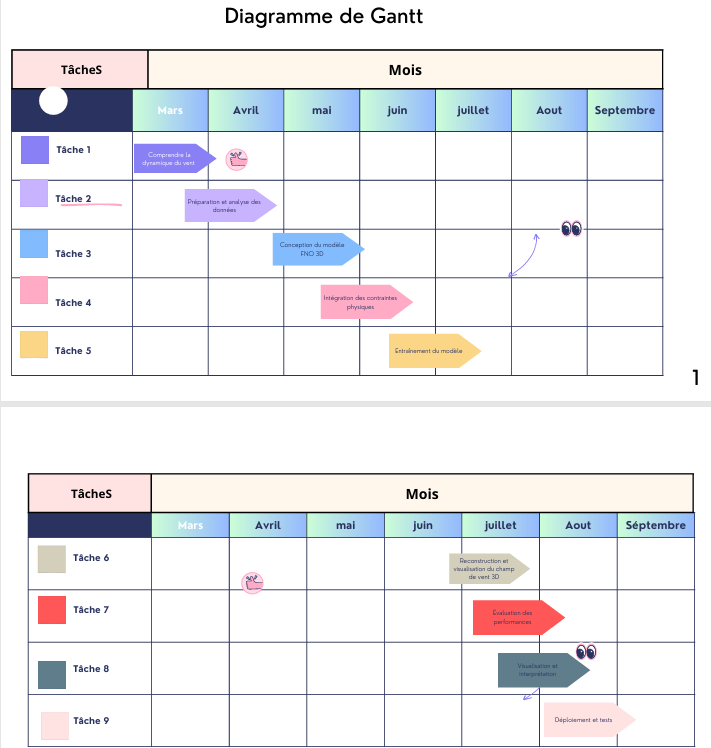
\includegraphics[width=0.82\linewidth]{figures/gantt_prevu.png}
  \caption{Diagramme de Gantt prévisionnel (mars--septembre 2026).}
  \label{fig:gantt}
\end{figure}

\subsection{Évolution du plan au fil des résultats}
Conformément au cycle TDSP, le plan a été adapté au fil des résultats
(tableau~\ref{tab:deroulement}). Une phase d'exploration large, qui a comparé six familles
d'architectures, a permis de converger vers un opérateur 3D unique ; la seconde moitié du projet,
organisée en lots courts terminés chacun par une mesure et une décision, a ensuite enchaîné le
modèle de référence, le passage aux données réelles, la mise en service et les études OS6 et OS7,
au-delà du périmètre prévu initialement.

\begin{table}[H]
\centering
\caption{Évolution du projet.}
\label{tab:deroulement}
\begin{tabularx}{\linewidth}{@{}p{3.2cm}X@{}}
\toprule
Période & Travaux\\
\midrule
mars -- juin 2026 & Étude de la dynamique du vent, génération des premières données ANEO, analyse exploratoire\\
juin -- sept. 2026 & Exploration de six familles d'architectures 2D (FNO 2D, U-Net/FNO, GNN, DeepONet, ResNet, ViT) ; extrapolation verticale séparée\\
fin sept. 2026 & Jeu synthétique 3D (\code{aneo\_dataset\_3d\_v2}, 12 niveaux) ; passage à un opérateur 3D supervisé directement\\
début oct. 2026 & Modèle de référence \textbf{v7} (140 époques, A100) ; portage du notebook en paquet Python testé\\
11 -- 16 oct. 2026 & Lots de clôture M0 à M8 : reproductibilité, fiabilité, contrat de données, alertes, éolien, publication, API, preuves ; tentative bornée M1 sur DSO1\\
21 -- 24 oct. 2026 & Domaine réel du Grand Tunis : générateur forcé par ERA5, modèles v1, v2, v2 prolongée, v3 (affinage sur stations, écarté), \textbf{v4} (livrée)\\
25 -- 31 oct. 2026 & Application ATOM Wind, temps réel GFS, cahier des charges v12, OS6 (plan du réseau)\\
nov. 2026 & OS7 (prévision +24/+48\,h) \acompleter{résultats à reporter}, rédaction\\
\bottomrule
\end{tabularx}
\end{table}

